\documentclass[preprint,12pt, a4paper]{elsarticle}

\usepackage{amssymb}
\usepackage{lineno}
\usepackage{float}
\usepackage{hyperref}
\usepackage{listings}
\lstset{language=Python}

\restylefloat{table}

\journal{SoftwareX}

\begin{document}

\begin{frontmatter}

\title{cluster-over-sampling: A package for clustering based oversampling}

\author{Georgios Douzas}
\ead{gdouzas@novaims.unl.pt}

\author{Fernando Bacao\corref{nova}}
\ead{bacao@novaims.unl.pt}

\address{NOVA Information Management School, Universidade Nova de Lisboa}

\cortext[nova]{Postal Address: NOVA Information Management School, Campus de Campolide, 1070-312 Lisboa, Portugal, Telephone: +351 21 382 8610}

\begin{abstract}
Learning from class-imbalanced data is a common and challenging problem in supervised learning. Standard classification algorithms are designed to handle balanced class distributions. While different strategies exist to tackle this problem, methods that generate artificial data to achieve a balanced class distribution, called oversampling algorithms, are more versatile than modifications to the classification algorithms. SMOTE algorithm, the most popular oversampler, as well as any other oversampling method based on it, generates synthetic samples along line segments that join minority class instances. SMOTE addresses only the issue of between-classes imbalance. On the other hand, by clustering the input space and applying any oversampling algorithm for each resulting cluster with appropriate resampling ratio, the within-classes imbalanced issue can be addressed. This approach, implemented in the cluster-over-sampling Python open source project, has been shown in various publications, using a variety of datasets, to outperform other standard oversamplers. In this paper we describe cluster-over-sampling in detail and make it available to the machine learning community. An important point is that the implementation integrates effortlessly with the Scikit-Learn ecosystem. Therefore, machine learning researchers and practitioners can integrate it directly to any pre-existing work.
\end{abstract}

\begin{keyword}
Machine learning \sep Classification \sep Imbalanced learning \sep Oversampling
\end{keyword}

\end{frontmatter}

\begin{table}[H]
\begin{tabular}{|p{6.5cm}|p{6.5cm}|}
\hline
Code metadata & \\
\hline
Current code version & v0.1.1 \\
\hline
Permanent link to code/repository used for this code version & \url{https://github.com/AlgoWit/cluster-over-sampling} \\
\hline
Legal Code License & MIT \\
\hline
Code versioning system used & git \\
\hline
Software code languages, tools, and services used & Python, Travis CI, AppVeyor, Read the Docs, Codecov, CircleCI, zenodo, Anaconda Cloud \\
\hline
Compilation requirements, operating environments \& dependencies & Linux, Mac OS, Windows \\
\hline
If available Link to developer documentation/manual & \url{https://cluster-over-sampling.readthedocs.io/} \\
\hline
Support email for questions & \href{mailto:georgios.douzas@gmail.com}{georgios.douzas@gmail.com} \\
\hline
\end{tabular}
\caption{Code metadata}
\label{} 
\end{table}

\linenumbers

%% main text

\section{Motivation and significance}
\label{motivation}

\subsection{Introduction}
\label{introduction}

The imbalanced learning problem is defined as a machine learning classification task using datasets with binary or multi-class targets where one of the classes, called the majority class, outnumbers significantly the remaining classes, called the minority class(es) \cite{Chawla2003}. Learning from imbalanced data is a frequent and non-trivial problem for academic researchers and industry practitioners alike. The imbalance learning problem can be found in multiple domains such as chemical and biochemical engineering, financial management, information technology, security, business, agriculture or emergency management \cite{Haixiang2017}.

The imbalanced learning problem describes the case where in a machine learning classification task using datasets with binary or multi-class targets, one of the classes, called the majority class, has a significantly higher number of samples compared to the remaining classes, called the minority class(es) \cite{Chawla2003}. Learning from imbalanced data is a non-trivial problem for both academic researchers and industry practitioners. Additionaly, imbalanced data can be frequently found in multiple domains such as chemical and biochemical engineering, financial management, information technology, security, business, agriculture or emergency management \cite{Haixiang2017}.

A bias towards the majority class is induced when imbalanced data are used to train standard machine learning algorithms. This results in low classification accuracy, especially for the minority class(es), when the classifier is evaluated on unseen data. An important measure for the degree of data imbalance is the Imbalance Ratio ($IR$), defined as the ratio between the number of samples of the majority class and each of the minority classes. Using a rare disease detection task as an example, with 1\% of positive cases corresponding to an $IR=\frac{0.99}{0.01}=99$, a trivial classifier that always labels a person as healthy will score a classification accuracy of 99\%. However in this case, all positive cases remain undetected. The observed values of $IR$ are often between 100 and 100.000 \cite{Chawla2002}, \cite{Barua2014}. Figure \ref{fig:imbalanced} presents an example of imbalanced data in two dimensions as well as the decision boundary identified by a typical classifier when they are used as a training set.

\begin{figure}[H]
	\centering
    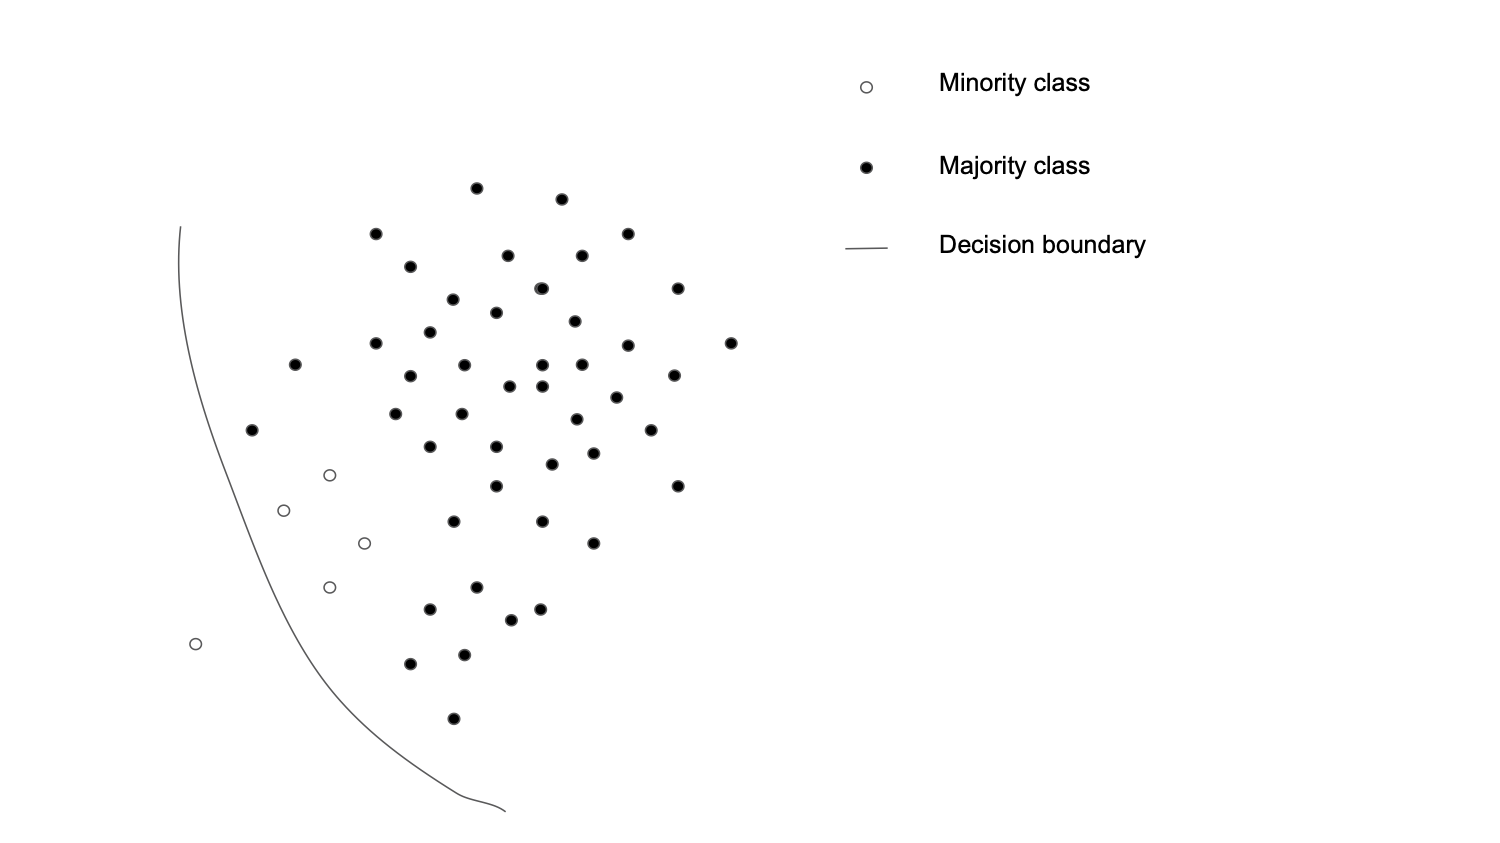
\includegraphics[width=14cm, keepaspectratio]{../analysis/imbalanced_problem}
    \caption{Imbalanced data in two dimensions. The decision boundary of a typical classifier shows a bias towards the majority class.}
    \label{fig:imbalanced}
\end{figure}

\subsection{Oversampling algorithms}
\label{oversampling}

Various approaches have been proposed to improve classification results when the training data are imbalanced, a case also known as between-class imbalance. The most general approach, called oversampling, is the generation of artificial data for the minority class(es) \cite{Fernandez2013}. Synthetic Minority Oversampling Technique (SMOTE) \cite{Chawla2002} was the first non-trivial oversampler proposed and remains the most popular one. Although SMOTE has been shown to be effective for generating artificial data, it also has some drawbacks \cite{He2009}. In order to improve the quality of the artificial data many variants of SMOTE have been proposed. Nevertheless, they utilize the SMOTE data generation mechanism, which consists of a linear interpolation between minority class samples to generate synthetic instances as shown in figure \ref{fig:smote}.

\begin{figure}[H]
	\centering
	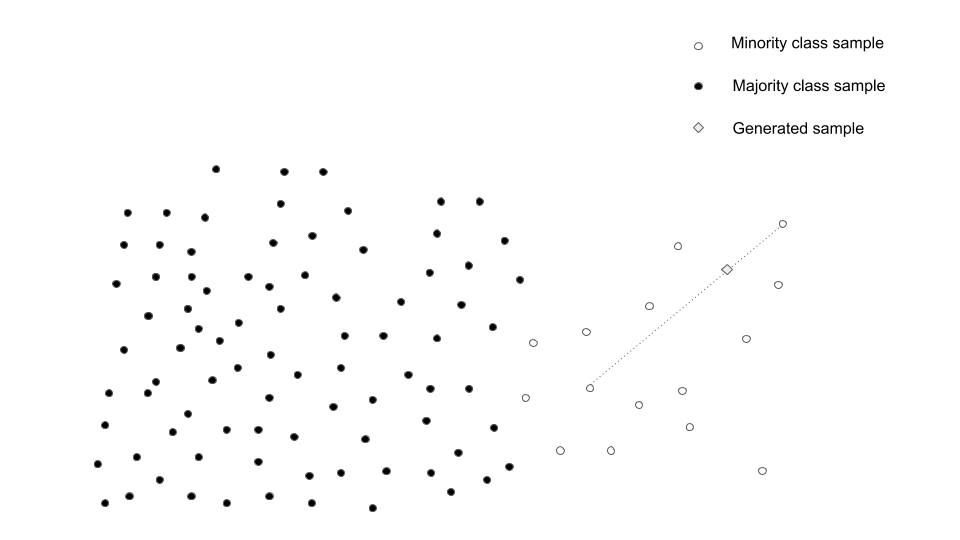
\includegraphics[width=1\linewidth]{../analysis/smote}
	\caption{Visual representation of the SMOTE data generation mechanism.}
	\label{fig:smote}
\end{figure}

A Python implementation of SMOTE and several of its variants is available in the \href{https://imbalanced-learn.org/stable/}{Imbalanced-Learn} \cite{Lemaitre2016} library, which is fully compatible with the popular machine learning toolbox \href{https://scikit-learn.org/stable/}{Scikit-Learn} \cite{Pedregosa2011}.

\subsection{Clustering based oversampling}
\label{clustering-oversampling}

In addition to between-class imbalance, within-class imbalance refers to the case where areas of sparse and dense minority class instances exist. As a first step of generating synthetic samples, the SMOTE data generation mechanism selects randomly, with uniform probability, minority class instances. Consequently, dense minority class areas have a high probability of being inflated further, while the sparsely populated are likely to remain sparse. This allows to combat between-class imbalance, while the issue of within-class imbalance is ignored \cite{Prati2004}.

On the other hand, clustering based oversampling, as presented in \cite{Douzas2017a} and \cite{Douzas2018}, aims to deal with both between-class and within-class imbalance problems. Initially a clustering algorithm is applied to the input space. The resulting clusters allow to identify sparse and dense minority class(es) areas. A small IR, compared to a threshold, of a particular cluster is used as an indicator that it can be safely used as a safe data generation area, i.e. noise generation is avoided. Furthermore, sparse minority clusters are assigned more synthetic samples, which alleviates within-class imbalance.

Specific realizations of the above approach are SOMO \cite{Douzas2017a} and KMeans-SMOTE \cite{Douzas2018} algorithms. Empirical studies have shown that both algorithms outperform SMOTE and its variants across multiple imbalanced datasets, classifiers and evaluation metrics. In this paper, we present a generic Python implementation of clustering based oversampling, in the sense that any combination of a Scikit-Learn compatible clusterer and Imbalanced-Learn combatible oversampler can be selected to produce an algorithm that identifies clusters on the input space and apply oversampling on each one of them.  In section 2, the software description is given while section 3 provides a demonstrative example of its functionalities.

\section{Software description}

The \texttt{cluster-over-sampling} software project is written in Python 3.7. It contains an object-oriented implementation of the cluster based oversampling procedure as well as detailed \href{https://cluster-over-sampling.readthedocs.io/}{online documentation}. The implementation provides an API that is compatible with Imbalanced-Learn and Scikit-Learn libraries. Therefore, standard machine learning functionalities are supported while the generated clustering based oversampling algorithm includes any selected oversampler as a special case.

\subsection{Software Architecture}
\label{architecture}

The \texttt{cluster-over-sampling} project contains the Python package \texttt{clover}. The main modules of \texttt{clover} are called \texttt{distribution} and \texttt{over\_sampling}. 

The module \texttt{distribution} implements the functionality related to the distribution of the generated samples to the identified clusters. It contains the files \texttt{base.py} and \texttt{density.py}. The former provides the implementation of the \texttt{BaseDistributor} class, the base class for distributors, while the later includes the \texttt{DensityDistributor} class, a generalization of the density based distributor presented in \cite{Douzas2017a} and \cite{Douzas2018}, that inherits from \texttt{BaseDistributor}. Following the Scikit-Learn API, \texttt{BaseDistributor} includes the public methods \texttt{fit} and \texttt{fit\_distribute}. The \texttt{fit\_distribute} method calls the \texttt{fit} method and returns two Python dictionaries that describe the distribution of generated samples inside each cluster and between clusters, respectively. Particularly, the \texttt{fit} method calculates various statistics related to the distribution process, while it calls \texttt{\_fit} method to calculate the actual intra-cluster and inter-cluster distributions. This is achieved by invoking the \texttt{\_intra\_distribute} and \texttt{\_inter\_distribute} methods. The \texttt{BaseDistributor} class provides a trivial implementation of them, that should be overwritten when a realization of a distributor class is considered. Therefore, \texttt{}{DensityDistributor} overwrites both methods as well as the \texttt{\_fit} method. The later calls the methods \texttt{\_identify\_filtered\_clusters} and \texttt{\_calculate\_clusters\_density} that identify the clusters used for data generation and calculate their density, respectively. Subsection \ref{functionality} provides a detailed description of the initialization and functionality of the \texttt{DensityDistributor} class. Figure \ref{fig:distributor_class_diagram} shows a visual representation of the above classes and functions hierarchy.

The initialization of a \texttt{GeometricSMOTE} instance includes G-SMOTE's hyperparameters that control the generation of synthetic data. Additionally, \texttt{GeometricSMOTE} inherits from the \texttt{BaseOverSampler} class of Imbalanced-Learn library. Therefore, an instance of \texttt{GeometricSMOTE} class provides the \texttt{fit} and \texttt{fit\_resample} methods, the two main methods for resampling as explained in subsection \ref{functionality}. This is achieved by implementing the \texttt{\_fit\_resample} abstract method of the parent class \texttt{BaseOverSampler}. More specifically, the function \texttt{\_make\_geometric\_sample} implements the data generation mechanism of G-SMOTE as shortly described in section \ref{clustering-oversampling}. This function is called in the \texttt{\_make\_geometric\_samples} method of the \texttt{GeometricSMOTE} class in order to generate the appropriate number of synthetic data for a particular minority class. Finally, the method \texttt{\_make\_geometric\_samples} is called in \texttt{\_fit\_resample} method to generate synthetic data for all minority classes. Figure \ref{fig:class_diagram} provides a visual representation of the above classes and functions hierarchy.

\begin{figure}[H]
	\centering
	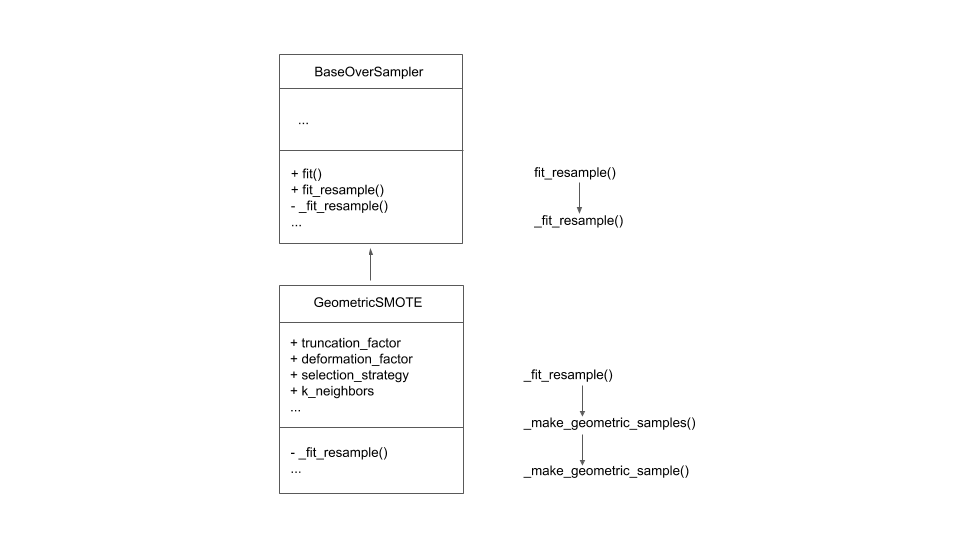
\includegraphics[width=1\linewidth]{../analysis/class_diagram}
	\caption{UML class diagrams and callgraphs of main classes and methods.}
	\label{fig:class_diagram}
\end{figure}

\subsection{Software Functionalities}
\label{functionality}

As it was mentioned in subsection \ref{architecture}, the class \texttt{GeometricSMOTE} represents the G-SMOTE oversampler. The intializer of \texttt{GeometricSMOTE} includes the following G-SMOTE's hyperparameters: \texttt{truncation\_factor}, \texttt{deformation\_factor}, \texttt{selection\_strategy} and \texttt{k\_neighbors} as explained in subsection \ref{gsmote}. Once the \texttt{GeometricSMOTE} object is initialized with a specific parametrization, it can be used to resample the imbalanced data represented by the input matrix \texttt{X} and the target labels \texttt{y}. Following the Scikit-Learn API, both \texttt{X}, \texttt{y} are array-like objects of appropriate shape.

Resampling is achieved by using the two main methods of \texttt{fit} and \texttt{fit\_resample} of the \texttt{GeometricSMOTE} object. More specifically, both of them take as input parameters the \texttt{X} and \texttt{y}. The first method computes various statistics which are used to resample \texttt{X} while the second method does the same but additionally returns a resampled version of \texttt{X} and \texttt{y}.

The \texttt{geometric-smote} project has been designed to integrate with the Imbalanced-Learn toolbox and Scikit-Learn ecosystem. Therefore the \texttt{GeometricSMOTE} object can be used in a machine learning pipeline, through Imbalanced-Learn's class \texttt{Pipeline}, that automatically combines \texttt{samplers}, \texttt{transformers} and \texttt{estimators}. The next section provides examples of the above functionalities.

\section{Illustrative Examples}

\subsection{Basic example}

An example of resampling multi-class imbalanced data using the \texttt{fit\_resample} method is presented in Listing \ref{lst:basic}. Initially, 
a 3-class imbalanced dataset is generated. Next, \texttt{GeometricSMOTE} object is initialized with default values for the hyperparameters, i.e. $\texttt{truncation\_factor} = 1.0$, $\texttt{deformation\_factor}=0.0$, $\texttt{selection\_strategy}=\textrm{combined}$. Finally, the object's \texttt{fit\_resample} method is used to resample the data. Printing the class distribution before and after resampling confirms that the resampled data \texttt{X\_res}, \texttt{y\_res} are perfectly balanced. \texttt{X\_res}, \texttt{y\_res} can be used as training data for any classifier in the place of \texttt{X}, \texttt{y}.

\begin{lstlisting}[caption={Resampling of imbalanced data using the \texttt{fit\_resample} method.},label={lst:basic}]
# Import classes and functions.
from collections import Counter
from gsmote import GeometricSMOTE
from sklearn.datasets import make_classification

# Generate an imbalanced 3-class dataset.
X, y = make_classification(
    random_state=23, 
    n_classes=3, 
    n_informative=5,
    n_samples=500,
    weights=[0.8, 0.15, 0.05]
)

# Create a GeometricSMOTE object with default hyperparameters.
gsmote = GeometricSMOTE(random_state=10)

# Resample the imbalanced dataset.
X_res, y_res = gsmote.fit_resample(X, y) 

# Print number of samples per class for initial and resampled data. 
init_count = list(Counter(y).values())
resampled_count = list(Counter(y_res).values())

print(f'Initial class distribution: {init_count}.') 
# Initial class distribution: [400, 75, 25].

print(f'Resampled class distribution: {resampled_count}.')
# Resampled class distribution: [400, 400, 400].
\end{lstlisting}

\subsection{Machine learning pipeline}

As mentioned before, the \texttt{GeometricSMOTE} object can be used as a part of a machine learning pipeline. Listing \ref{lst:pipeline} presents a pipeline composed by a G-SMOTE oversampler, a PCA tranformation and a decision tree classifier. The pipeline is trained on imbalanced binary-class data and evaluated on a hold-out set. The user applies the process in a simple way while the internal details of the calculations are hidden.

\begin{lstlisting}[caption={Training and evaluation of a machine learning pipeline that contains the \texttt{GeometricSMOTE} object.},label={lst:pipeline}]
# Import classes and functions.
from gsmote import GeometricSMOTE
from sklearn.datasets import make_classification
from sklearn.decomposition import PCA
from sklearn.tree import DecisionTreeClassifier
from sklearn.model_selection import train_test_split
from sklearn.metrics import f1_score
from imblearn.pipeline import make_pipeline

# Generate an imbalanced binary-class dataset.
X, y = make_classification(
	random_state=23, 
	n_classes=2, 
	n_samples=500,
	weights=[0.8, 0.2]
)

# Split the data to training and hold-out sets.
X_train, X_test, y_train, y_test = train_test_split(X, y, random_state=0)

# Create the pipeline's objects with default hyperparameters.
gsmote = GeometricSMOTE(random_state=11)
pca = PCA()
clf = DecisionTreeClassifier(random_state=3)

# Create the pipeline.
pip = make_pipeline(gsmote, pca, clf)

# Fit the pipeline to the training set.
pip.fit(X_train, y_train)

# Evaluate the pipeline on the hold-out set using the F-score.
test_score = f1_score(y_test, pip.predict(X_test))

print(f'F-score on hold-out set: {test_score}.')
# F-score on hold-out set: 0.7.
\end{lstlisting}

\section{Impact and conclusions}

Classification of imbalanced datasets is a challenging task for standard machine learning algorithms. G-SMOTE, as a enhancement of the SMOTE data generation mechanism, provides a flexible and effective way for resampling the imbalanced data. G-SMOTE's emprical results prove that it outperforms SMOTE and its variants. Machine learning researchers and industry practitioners can benefit from using G-SMOTE in their work since the imbalanced learning problem is a common characteristic of many real-world applications.

The \texttt{geometric-smote} project provides the only Python implementation, to the best of our knowledge, of the state-of-the-art oversampling algorithm G-SMOTE. A significant advantage of this implementation is that it is built on top of the Scikit-Learn's ecosystem. Therefore, using the G-SMOTE oversampler in typical machine learning workflows is an effortless task for the user. Also, the public API of the main class \texttt{GeometricSMOTE} is identical to the one implemented in Imbalanced-Learn for all oversamplers. This means that users of Imbalanced-Learn and Scikit-Learn, that apply oversampling on imbalanced data, can integrate the \texttt{gsmote} package in their existing work in a straightforward manner or even replace directly any Imbalanced-Learn's oversampler with \texttt{GeometricSMOTE}.

\section{Conflict of Interest}

We wish to confirm that there are no known conflicts of interest associated with this publication and there has been no significant financial support for this work that could have influenced its outcome.

\bibliography{references}
\bibliographystyle{elsarticle-num}
\end{document}
\endinput

